\section{Our approach: {\orirrp}} \label{sec:solution}
{\rrp} is an modified A* algorithm with additional graph pruning power. {\rrp} consists of two main components, spatial and social components. Spatial components includes a grid-based index for pruning graph branches while the social components use landmark techniques to generate distance heuristic for guiding graph traversal. In the following, we explain the two components of {\rrp} in details.
%The solution is two fold, first data is preprocessed to create an index. Then a modified A* algorithm traverses the graph using the index to answer query of type mentioned in Section \ref{sec:preliminary}.

% Throughout the section, a running example is used to explain the main idea followed by a formal algorithm. Consider Figure \ref{fig:running-example-solution} which has a social graph of friends and their check-ins at various venues. In Figure \ref{fig:running-example-solution}, each vertex symbolizes a person and two nodes are connected if there is a social relationship between them. The number on the edge indicates their social distance, lesser implies stronger bond. Forest green edges from the nodes to the map are all check-ins made by people at various venues (nodes not shown), which are our spatial vertices. Forest green edges are also weighted but are not shown as they are not important for explanation purposes.

\begin{figure}[t]
	\centering 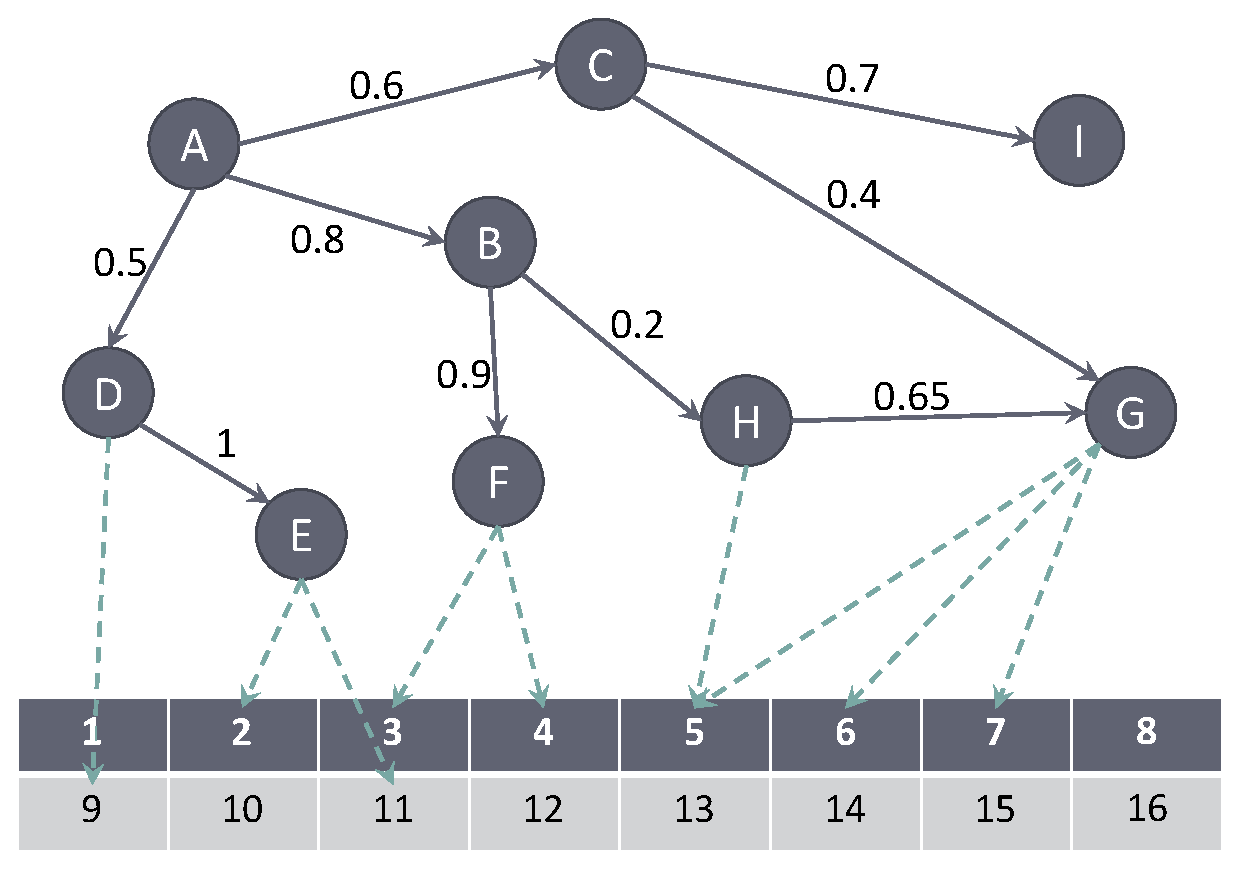
\includegraphics[width=0.40\textwidth]{images/space_partitioned_world.eps}
    \caption{Running Example}
    \label{fig:running-example-solution}
\end{figure}

%\subsection{Index Structure}
%Goal of the index is to quickly prune the graph for any range predicate, starting at any source vertex. Therefore for every vertex, spatial and social meta information is added. Using this meta information, the traversal algorithm at query time can decide whether to visit a sub-graph starting at that node or not or more generally, this guides the traversal algorithm at query time.

%Spatial meta information is created using the spatial attributes of the vertices. The world is divided into a fixed number of blocks in space and are numbered in increasing order. Then for each venue (i.e. spatial node) the meta information for all the people nodes (other vertices) who have directly and indirectly checked-in there is updated with the block number where the venue belongs. 

% If the world is divided into very fine blocks, each meta entry can be really huge. To compress the index entry, the world is divided again but this time into more coarser blocks and are also numbered like before. For all the index entries which cross a threshold, block numbers from the coarser division are used. This is done recursively until the threshold is satisfied for that index entry. Once this is in place, at query time, while traversing the graph for finding a closest vertex, sub-graphs starting at a vertex which does not reach the region of interest are straight away pruned.

%Social meta information/index is created using the social distances (edge weights). A few vertices are picked from the graph and the shortest distances from each to all vertices it can reach are stored. Using these vertices and triangle inequality an estimate of the shortest distance from any vertex to any other vertex in the graph is obtained.

\subsection{Spatial Component}

\begin{figure}[t]
	\centering \includegraphics[width=0.40\textwidth]{images/entire_world_grid.eps}
    \caption{Space partitioned world}
    \label{fig:space-partitioned}
\end{figure}

A complete picture of equally space partitioned world would be as shown in the Figure~\ref{fig:space-partitioned}. Here the resolution of the division is 10 by 10. That means the entire world is divided into 10 equal sized blocks horizontally and 10 equal sized blocks vertically. In the running example, the entire region is divided into equal sized blocks from 1 to 16 as shown in Figure \ref{fig:running-example-solution}. Then for vertex D, meta information would be [8] as the user checked-in at a venue which falls in block number 8. Similarly for vertex G, the meta information would be [5, 6, 7]. Continuing like this, a meta information table for each vertex which are directly connected to a spatial node is populated.

% \begin{table}[h]
% 	\caption{1-hop reachability meta table}
% 	\label{tab:1-hop-meta}
% 	\begin{center}
% 		\renewcommand{\arraystretch}{1.25}
% 		\begin{tabular}{ c | c }
% 			\hline
% 			Vertex & Reachable Block Numbers \\ \hline
% 			\hline
% 			D & [8] \\
% 			E & [2, 10] \\
% 			F & [3, 4] \\
% 			H & [5] \\
% 			G & [5, 6, 7] \\
% 			\hline
% 		\end{tabular}
% 	\end{center}
% \end{table}

% This is the reachability to venues by 1-hop which can answer 1-hop queries. For example, did vertex G check-in at venue L1 or did vertex E visit any venue in a region L2. The first can be answered by finding its block number using its location and cross-reference it with the list of blocks G can reach from the meta table. More details on answering queries are in Section \ref{querying}.

% If idea of 1-hop reachability is extended to any number of hops, it is multi-hop reachability or simply reachability. These values denote all blocks that are reachable from a vertex in any number of hops/steps. 

Now to complete building the reachable block table, direction of all the edges are reversed or the transpose of a graph is created. Then, for every vertex, its reachability information is appended with meta information of all the vertices it is directly connected to bottom up. In the example after reversing the edges, to compute multi-hop meta information for H, append G's meta information to it. Similarly for B's meta information is appended from H and F. As this is a DAG, this is the complete reachability information of every node after completing the exercise for entire graph. If the original graph is not a DAG, it is condensed by contracting all strongly connected components into a single node to make it a DAG. The final meta table for every node looks like the one shown in the column 2 of Table \ref{tab:multi-hop-meta}.

\begin{table}[h]
	\caption{Meta table for multi-hop reachability}
	\label{tab:multi-hop-meta}
	\begin{center}
		\renewcommand{\arraystretch}{1.25}
		\begin{tabular}{ c | c | c }
			\hline
			Vertex & Reachable Block Numbers & Compressed\\ \hline
			\hline
			D & [9, 2, 11] & [17, 18] \\
			E & [2, 11] & [2, 11] \\
			F & [3, 4] & [3, 4] \\
			H & [5, 6, 7] & [19, 20] \\
			G & [5, 6, 7] & [19, 20] \\
			C & [5, 6, 7] & [19, 20] \\
			B & [3, 4, 5, 6, 7] & [21] \\
			A & [3, 4, 5, 6, 7] & [21] \\
			\hline
		\end{tabular}
	\end{center}
\end{table}

Using this table any region reachability query can be answered and will be described in Section \ref{querying}. Now it can seen that vertex A can reach whatever B, C and D can reach. Similarly B can reach whatever H and F can reach and so on. However, as you can see the size of the meta table (a.k.a index table) can grow really large as vertices like B and A which are highly connected can reach many blocks.

In order to compress the entries in the meta table for highly reachable nodes, a new layer of blocks with higher resolution is added.

% \begin{figure}[h]
%     \centering
%     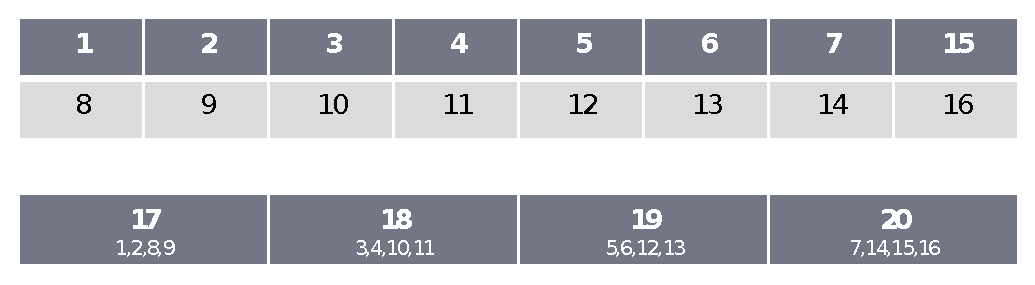
\includegraphics[width=0.8\linewidth]{images/image07.eps}
%     \caption{Multi layer grid index}
%     \label{fig:multi-grid}
% \end{figure}

As shown in Figure \ref{fig:multi-grid2} (assume the 3rd layer does not exist for now), blocks 17 to 20 are added on top of blocks 1 to 16. This can be visualized like a stack where the old layer sits exactly on top of the new layer. That is block 17 covers exactly the same area as area covered by blocks 1, 2, 8 and 9. Similarly block 18 in layer 1 represents blocks 3, 4, 10 and 11 of layer 0. Due to this change, the meta table becomes like the one shown in the 3rd column of the Table \ref{tab:multi-hop-meta}. The reduction factor, which is rate at which the resolution changes between adjacent layers, is set to 1/4 and is a tunable parameter of the system called RF. The number of layers in the multi layer grid index is guided by another system level tunable parameter M. M is the maximum size, in terms of number of block ids, of meta information for a vertex. For example, if M = 2 as used in the running example, then each vertex can only have two entries in its meta information and until this limit is satisfied, new layers are created. In the example, for all vertices which have more than 2 entries, are compressed using layer 1. However some of them still have more than 2 entries. 

% \begin{table}[h]
% 	\caption{Compressed Meta table for multi-hop reachability}
% 	\label{tab:multi-hop-meta-compressed}
% 	\begin{center}
% 		\renewcommand{\arraystretch}{1.25}
% 		\begin{tabular}{ c | c }
% 			\hline
% 			Vertex & Reachable Block Numbers \\ \hline
% 			\hline
% 			D & [8] \\
% 			E & [2, 10] \\
% 			F & [3, 4] \\
% 			H & [\textbf{19, 20}] \\
% 			G & [\textbf{19, 20}] \\
% 			\textbf{C} & [\textbf{19, 20}] \\
% 			\textbf{B} & [\textbf{18, 19, 20}] \\
% 			\textbf{A} & [\textbf{18, 19, 20}] \\
% 			\hline
% 		\end{tabular}
% 	\end{center}
% \end{table}

To compress further one more layer below layer 1 is added as show in Figure \ref{fig:multi-grid2}. There block 21 represents blocks 17, 18, 19 and 20 in the layer above it. 

\begin{figure}[t]
    \centering
    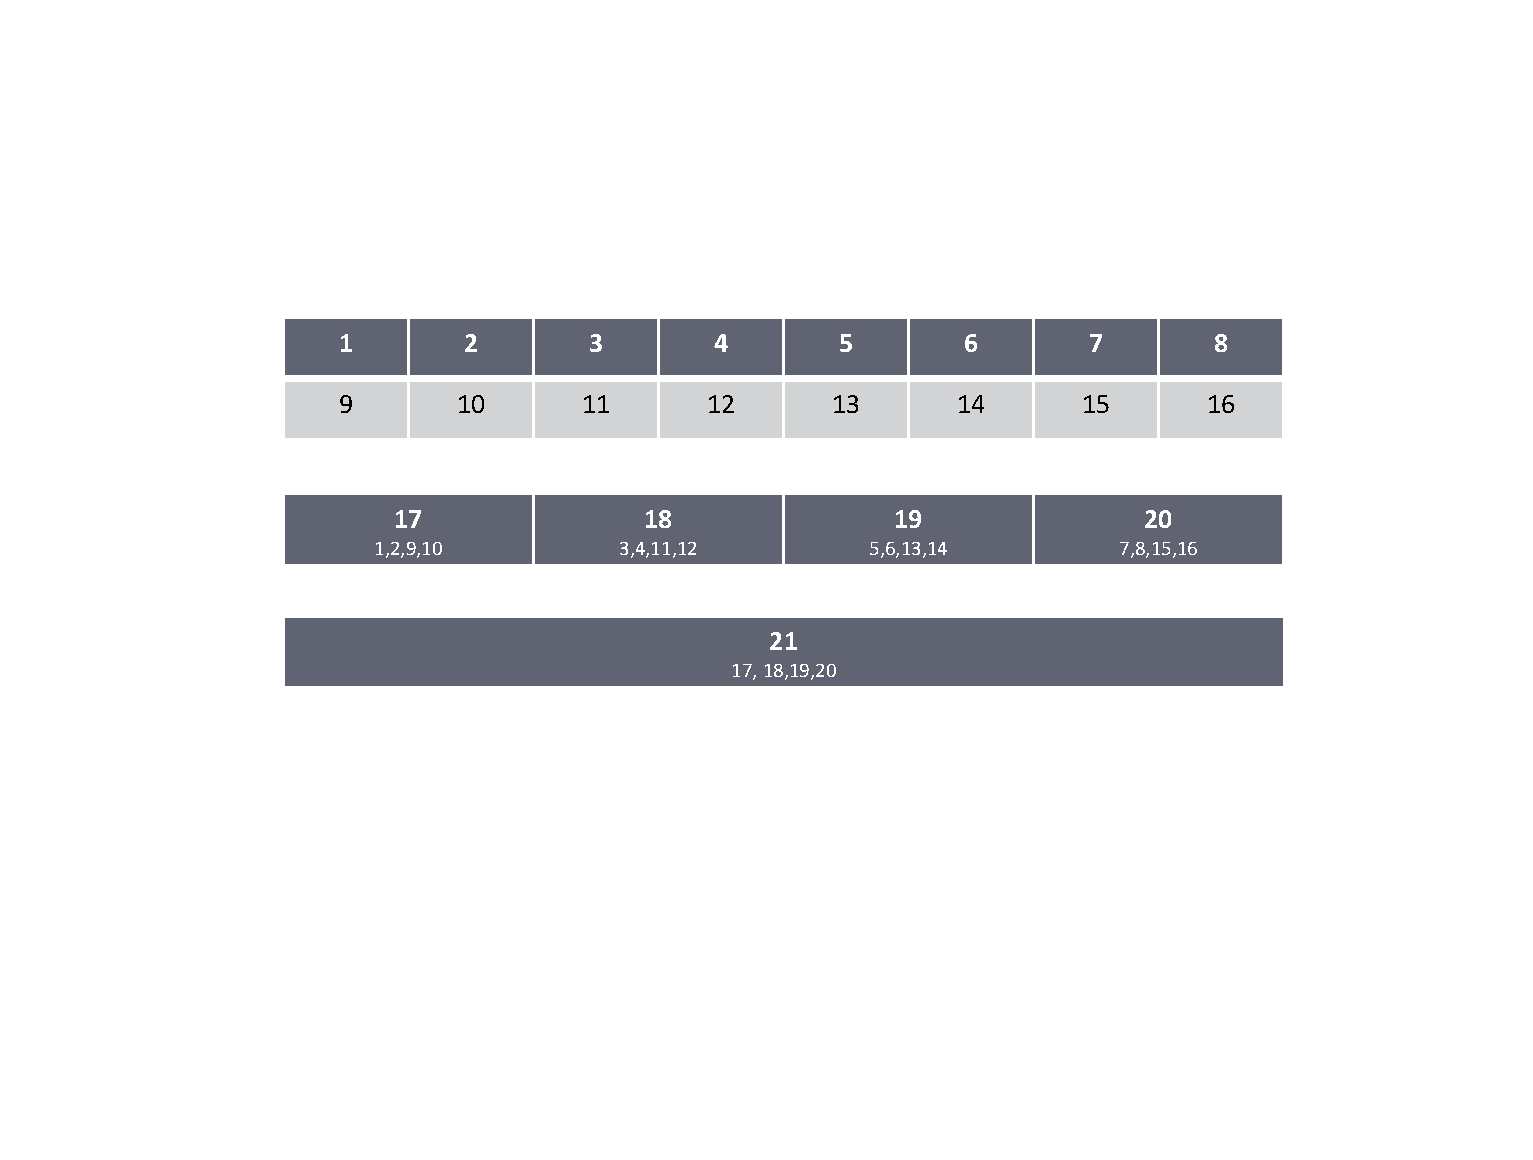
\includegraphics[width=0.88\linewidth]{images/multi_layer_grid_index.eps}
    \caption{Multi layer grid index}
    \label{fig:multi-grid2}
\end{figure}

The discussion began by condensing G to a DAG (G'). Now each node in a strongly connected component gets the meta information of the component as proved Lemma \ref{vertex-component-meta}.

\begin{lemma}
\label{vertex-component-meta}
Let v be a vertex in a strongly connected component C of a directed graph G(V, E). Then,

{\{$\forall v \in C$: Meta information of v = Meta information of C\}}\\
\end{lemma}

\begin{proof}
In a strongly connected component $C$, any vertex can be reached from any vertex by definition, i.e. $u \leadsto v, \forall (u, v) \in C$. 

If $C$ in condensed graph $G'$ can reach a set of regions $R$, then any vertex of $C$ can reach $R$ by definition of connected component.

Therefore, meta information of $C =$ meta information of $\forall v \in C$
\end{proof}

Then a R-Tree is also constructed using the spatial nodes in the graph. This will later be used at query time to filter the exact nodes in a region and will be discussed in more details in Section \ref{querying}. R-Tree index and reachable blocks table are the two indices created on the spatial component of the graph.

Algorithm \ref{alg1} shows how the index, {\rrpspatial} is created. In the first phase block numbers of all spatial vertices are added as the meta information of the vertices they are connected from. Then a modified DFS is used to construct multi hop reachability. The REGION() method returns the block number for any spatial vertex. The REPARTITION() method ensures the M constraint by recursively increasing the resolution by a factor of RF. In the DFS() method meta information is recursively appended to the head vertex from the tail vertex.

% \begin{algorithm*}[h]
% \caption{{\grpspatial}}
% \label{alg1}
% \begin{multicols}{2}
% \begin{algorithmic}[1]
% \State $MIN\_LAT \gets -90$
% \State $MAX\_LAT \gets 90$
% \State $MIN\_LNG \gets -180$
% \State $MAX\_LNG \gets 180$
% \State $DEFAULT\_RES \gets 10$ \Comment{Can be any positive integer}
% \State $AVAILABLE\_RES \gets [DEFAULT\_RES]$
% \State
% \Function{{\grpspatial}}{$G, RF, M$}
%   \State $G' \gets DAG(G)$
%   \For{$v \gets G'.v:$}
%   	\State $v.meta \gets Set([])$   	\Comment{Initialize an empty set}
%   \EndFor
%   \State
%   \For{$u \gets spatial(G'.Adj(v))$}	 \Comment{1\-hop spatial reachability}
%   	\State v.meta.add(\Call{REGION}{u})
% 	\State \Call{REPARTITION}{v, RF, M}
%   \EndFor
%   \State
%   \State DO\_DFS(G', RF, M)  \Comment{multi\-hop region reachability}
% \EndFunction
% \State
% \Function{REGION}{$u$}
% 	\State $r \gets GET\_RES(u)$
% 	\State $cols \gets (MAX\_LAT - MIN\_LAT) \div r$
% 	\State \Return $floor(u.x \div r) + floor(u.y \div r)$
% \EndFunction
% \State
% \Function{REPARTITION}{$v, RF, M$}
% 	\If{$v.meta.size() \leq M$}
% 		\State \Return
% 	\EndIf
% 	\State $res \gets GET\_RES(v.meta[0])$
% 	\For{$r \gets v.meta$}
% 		\State \Call{TRANSLATE\_TO\_RES}{v.meta, $res \div MF$}
% 		\State \Call{REPARTITION}{v, RF, M}
% 	\EndFor
% \EndFunction
% \State
% \Function{DO\_DFS}{G, RF, M}
% 	\For{$v \gets G,V$}
% 		\State $v.visited \gets false$
% 	\EndFor
% 	\State
% 	\For{$v \gets G.V$}
% 		\State v.meta.add(\Call{DFS\_VISIT}{G, v})
% 		\State \Call{REPARTITION}{v, RF, M}
% 	\EndFor
% \EndFunction
% \State
% \Function{DFS\_VISIT}{G, v}
% 	\For{$u \gets G.Adj(v)$}
% 		\If{$v.visited = false$}
% 			\State v.meta.add(\Call{DFS\_VISIT}{G, u})
% 		\Else
% 			\State v.meta.add(u.meta)
% 		\EndIf
% 		\State \Call{REPARTITION}{v, RF, M}
% 		\State $v.visited \gets true$
% 		\State \Return v.meta
% 	\EndFor
% \EndFunction
% \end{algorithmic}
% \end{multicols}
% \end{algorithm*}

\begin{algorithm}[t]
\caption{{\rrpspatial} Initialization}
\begin{scriptsize}
\label{alg1}
\begin{algorithmic}[1]
\Function{{\inirrpspatial}}{$G, RF, M$}
  \State G' $\gets$ G.condense() \label{alg:condense}
  \For{v $\gets$ G.V} \Comment{1\-hop spatial reachability} \label{alg:onehopstart}
	  \For{u $\gets$ spatial(G'.Adj(v))}	 
	  	\State v.meta.add(\Call{REGION}{u})
	  \EndFor
	  \State \Call{REPARTITION}{v, RF, M}
  \EndFor \label{alg:onehopend}
  \State DO\_DFS(G', RF, M)  \Comment{multi\-hop region reachability} \label{alg:dfs}
\EndFunction
\Function{REGION}{$u$}
	\State \Return block \# for CURRENT\_RES(u)
\EndFunction
\Function{REPARTITION}{$v, RF, M$}
	\While{$v.meta.size() \leq M$}
		\State \Call{TRANSLATE\_TO\_RES}{v.meta, CURRENT\_RES(v) $\div$ RF}
	\EndWhile
\EndFunction
\Function{DO\_DFS}{G, RF, M}
	\For{$v \gets G.V$}
		\State v.meta.add(\Call{DFS\_VISIT}{G, v})
		\State \Call{REPARTITION}{v, RF, M}
	\EndFor
\EndFunction
\Function{DFS\_VISIT}{G, v}
	\For{$u \gets G.Adj($v) not $visited$}
		\State v.meta.add(\Call{DFS\_VISIT}{G, u})
	\EndFor
	\State \Return v.meta
\EndFunction
\end{algorithmic}
\end{scriptsize}
\end{algorithm}

To compute the asymptotic run time and space complexities for Algorithm \ref{alg1}, it is divided into four pieces - graph condensation, reachability and repartition function. The runtime for each would be as follows,
\begin{itemize}

  \item \textbf{Graph Condensation}: On Line~\ref{alg:condense}, the input graph is condensed into its strongly connected components. Using a popular algorithm like Targan's Algorithm, the runtime would be $O(V + E)$~\cite{R1972}.

  \item \textbf{Reachability calculation}: From lines~\ref{alg:onehopstart} to~\ref{alg:dfs}, reachability on the condensed graph is computed. In the worst case, every vertex will be a strongly connected component and so the size of the graph remains the same after graph condensation. As the entire graph is traversed once to populate meta data for each vertex, the complexity for this piece also would be $O(V + E)$. Calls to repartition() function are handled separately.

  % \item \textbf{DFS}: For multi-hop reachability, a DFS traversal is performed on the graph on Line~\ref{alg:dfs}. As adjacency list is used for managing the graph's edges, the complexity for DFS would be $O(V + E)$ again. Calls to repartition() function are handled separately.

  \item \textbf{Repartition}: This function is called multiple times to make sure the M constraint is satisfied. The runtime of the function depends on the size of the meta entry for the vertex. For every vertex's index entry, the world is divided with a constant resolution to start with, like 10. The total number of blocks at that default resolution would always be square of it, like 100. Let the total number of blocks in the default resolution be $c$, which would be the worst case size of any vertex's meta information. This happens when a vertex can reach all blocks in the world. And until the size of meta information for that vertex falls below M, the resolution of the division is reduced by $RF$. Therefore the number of times the loop in REPARTITION() function of the algorithm, say $n$ would be,

  \begin{eqnarray*}
  	\dfrac{c}{RF^n} \leq M\\
  	n \leq {\log_{\dfrac{1}{RF}} (\dfrac{M}{c})}
  \end{eqnarray*}
  And repartition function is called exactly twice for each vertex, once during 1-hop reachability and once during DFS. Therefore, the time complexity due to this function would be $O(V \times {\log_{\dfrac{1}{RF}} (\dfrac{M}{c})})$. This fraction is very small compared to sum of vertices and edges in the graph.
\end{itemize}

All the other lines in the algorithm can be computed in constant time. The runtime of {\rrpspatial} would hence be $O(V + E)$.

Space complexity would be amount of memory required to store the multi-hop reachability table. Each index entry has an upper bound of $M$. Hence memory consumption in the worst case would be, $O(V \times M)$.

\subsection{Social component}
Social distances between nodes are used to create an additional index to prune the graph even better. This will take care of the cases when the graph is very dense and the spatial reachable blocks table created before may not be of much use for pruning at query time. More details on querying the graph are described in the next section.

The main idea is to select a few nodes in the graph and call them landmarks. Then for each vertex shortest distances to each landmark is stored. Then at query time these precomputed distances and triangle inequality are used to guide as a heuristic in the A* search algorithm. The inspiration is from \cite{AC2005} which introduces a class of algorithms called ALT. The main challenge here however is to find top-k closest vertices to a given vertex in a region and not finding the shortest path from a given source to a given destination unlike in \cite{AC2005}.

The quality of the landmarks determine the pruning power of the index. Choosing the right landmarks requires some domain knowledge of the graph. Once that is picked the process remains the same no matter what the graph represents. \cite{AC2005} talks about multiple ideas on how to find high quality landmarks quickly. The ideal case would be to find as minimum number of landmarks as possible such that every vertex in the graph is connected to at least one of the landmarks.  However leaving out a few vertices that do not reach any landmarks will not hamper the correctness of the algorithm. Therefore finding a sweet spot of number of landmarks which gives the best query performance is crucial and is the main goal of \cite{AC2005}. The main contribution from our side is to use {\rrpsocial} and propose a new heuristic for A* algorithm that finds topK venues satisfying a spatial predicate.

Algorithm \ref{alg2}, {\rrpsocial}, describes how to create an index using landmarks. Landmark selection function on line 2 can be any of the functions described in \cite{AC2005}. Then for each landmark the shortest distances is computed using any well-known single source shortest path algorithms like Dijkstra's or Bellman Ford to every vertex reachable from that landmark. Please note that distances from the landmark to every vertex are saved and not the other way around. The direction is important as directed graphs are only dealt here.

\begin{algorithm}[t]
\caption{{\rrpsocial}  Initialization}
\begin{scriptsize}
\label{alg2}
\begin{algorithmic}[1]

\Function{{\inirrpsocial}}{$G$}
  \State L $\gets$ FIND\_LANDMARKS(G) \Comment{Domain based}
  \State social\_index $\gets$ []
  \For{l $\gets$ L}
    \For{v $\gets$ G.v}
	  	\State social\_index[l][v] $\gets $ shortest distance from l to v
	\EndFor
  \EndFor
\EndFunction
\end{algorithmic}

\end{scriptsize}
\end{algorithm}

To compute asymptotic run time and space complexities, Algorithm \ref{alg2} is divided into two pieces - finding the landmarks, finding shortest distances to each reachable vertex from each landmark. The runtime for each is as follows,
\begin{itemize}
	\item \textbf{Finding Landmarks}: There are various ways of picking the landmarks and is totally left to user. In our case we used an approach which finds landmarks in constant number of scans of the entire graph. Therefore, the complexity of this piece is $O(V + E)$.

	\item \textbf{Shortest distance to each landmark}: Here, the shortest distances from each landmark to all vertices it can reach are saved. Using adjacency list for storing the edges, Dijkstra's algorithm is used as edges have positive weights. With this setting, the complexity would be $O(landmarks \times E\log V)$. As the number of landmarks is usually very small compared to number of edges in the graph, it would be $O(E\log V)$ in asymptotic notation.
\end{itemize}

Therefore the runtime for this algorithm using a sensible landmark selection algorithm would be, $O(V + E) + O(E\log V)$.

Space complexity would be memory taken to store the shortest distances to each reachable vertex for all landmarks. As the number of landmarks is very small compared to the number of vertices in the graph, this would be $O(V)$.

\subsection{Query Processing} \label{querying}

A modified A* with landmark~\cite{AC2005} algorithm is proposed for answering {\query} queries using the {\grp} index ({\rrp}). The main goal is to prune as much graph as possible using the spatial reachable blocks table and move in a goal oriented manner towards the region during traversal. The algorithm takes a graph G, a starting vertex s and a query rectangle R as input and returns the top-K vertices by social distance in R in an iterative manner. Being iterative helps pipeline the {\rrp} with other database functions.

The crux of A* algorithm is the heuristic function. Our heuristic function takes a vertex and a region and returns the heuristic distance which will be used by A* to decide which path to traverse. In order to design such heuristic function {\rrpsocial} index is used explained in Algorithm \ref{alg3}. For this the triangle inequality property is used to get a lower bound on the distance between any two vertices.

In Figure \ref{fig:tri-ine}, say $H$ and $R$ vertices need a lower bound on the distance between them. For this, the distances saved w.r.t. each landmark, here $G$ as part of social {\rrp} index is used. So in the figure using the index the distances \textbf{u} and \textbf{v} are known. In order to find \textbf{x} which is the distance between $H$ and $X$ \textbf{u} is subtracted from \textbf{v}. Therefor the value of \textbf{x} shown in the figure would be $\textbf{v} - \textbf{u}$ which directly follows from vector addition. This is only a lower bound on the distance from $H$ to $X$ and is proved in \cite{AC2005}.

In our case a lower bound from a vertex to a region is needed. In order to understand how this is done, recap the problem definition - find top-k closest vertices (w.r.t social distances) in a region from a vertex in a graph. To understand better, set K = 1, i.e. say the nearest vertex in the R from a source vertex is needed and say only one landmark is present. Now, for A* to work efficiently, a lower bound as tight as possible is needed, else the traversal would touch as many vertices as Dijkstra's. Let the source vertex be $H$, landmark be $G$ and region exactly enclosing blocks 5 and 6 in the Figure \ref{fig:tri-ine}. The problem now becomes finding the closest vertex to $H$ in the region. To get a lower bound for $\textbf{x}$, the triangle inequality formula devised above, $\textbf{v} - \textbf{u}$ is used. In order to keep $\textbf{x}$ minimum, $\textbf{v}$ should be as small as possible. Therefore the closest vertex in R to $G$ is picked. Similarly for the second closest vertex the second nearest vertex to $G$ in R is chosen. The algorithm proceeds this way till the nearest K vertices in R are found. If multiple landmarks are present, a value of \textbf{x} for each landmark is produced. The maximum value of \textbf{x} is picked to get the tightest bound possible and this follows from efficiency of A* algorithm.

\begin{figure}[t]
    \centering
    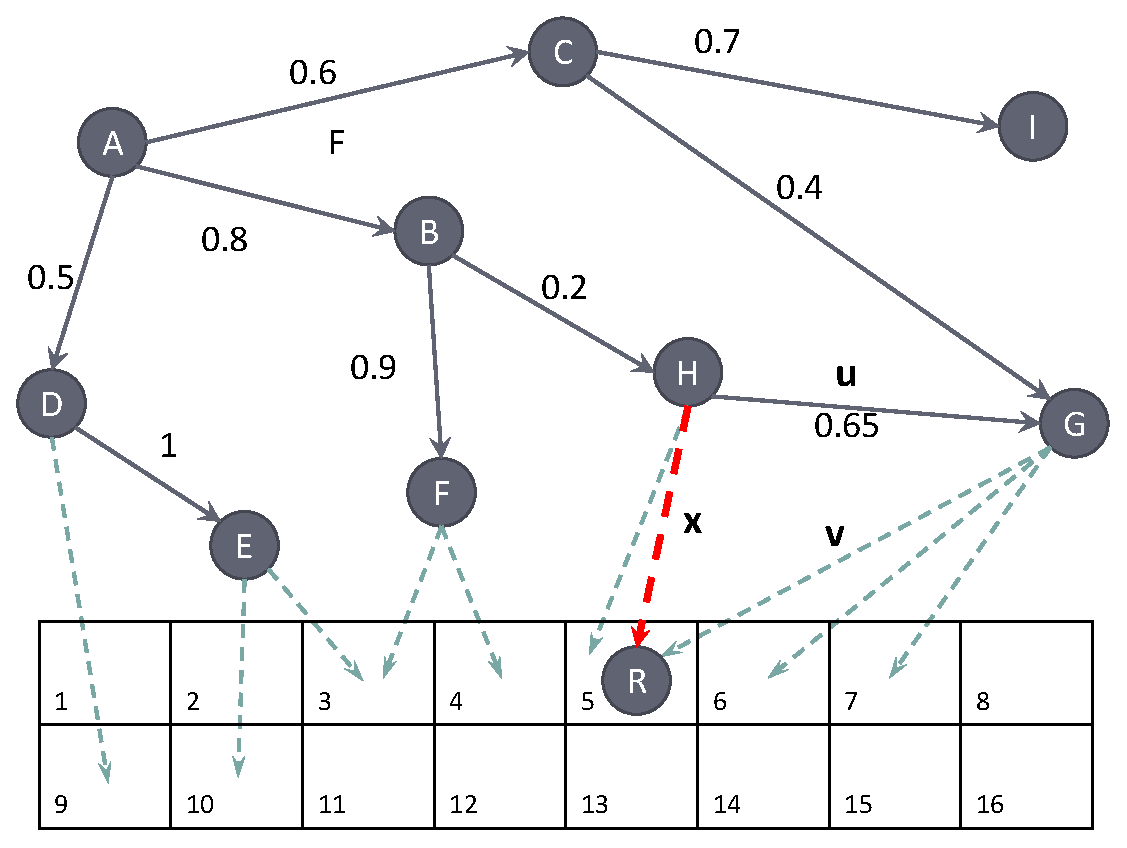
\includegraphics[width=0.88\linewidth]{images/triangle_inequality.eps}
    \caption{Triangle Inequality}
    \label{fig:tri-ine}
\end{figure}

Algorithm \ref{alg3} shows how to solve {\query} by using {\rrp} in detail. All vertices are labelled as unvisited initially. The visited flag is used to prevent traversing the same node multiple times. The priority queue $Q$ in keyed by sum of actual distance from source and a heuristic distance to current closest vertex to a landmark. For each vertex popped from the queue, it is tested if it lies in R and returned if K vertices are found. If not, keys for all existing vertices in Q are updated with the new heuristic. All unvisited neighbors of the popped vertex are enqueued only if they can reach the region R as per {\rrpspatial} index. If a neighbor can reach R, and if it not already in $Q$, its heuristic distance is computed and summed with the distance from the source and inserted into the $Q$. If the vertex is already in the $Q$, its key is updated if the new distance is smaller. The algorithm proceeds this way till all vertices in the Q are exhausted or K closest vertices in R are found whichever is earlier. This way, it is an iterative algorithm which doesn't traverse the entire graph to return the top-K results.

% \begin{algorithm*}[h]
% \caption{RangeReachPaths}
% \label{alg2}
% \begin{multicols}{2}
% \begin{algorithmic}[1]
% \Function{{\rrp}}{G, s, R, K}
% 	\State $nearest\_vertices \gets []$
% 	\State \Call{INIT}{G, s}
% 	\State $Q \gets [s]$
% 	\State $best\_index \gets 0$
% 	\While{Q is not empty}
% 		\State $v \gets \Call{EXTRACT\_MIN}{Q}$
		
% 		\If{\Call{LIES\_IN}{v, R}}
% 			\State $nearest\_vertices << v$ \Comment{add v to set}
% 			\State $best\_index \gets best\_index + 1$
% 			\If{nearest\_vertices.length = K}
% 				\State \Return \Call{PATHS}{nearest\_vertices}
% 			\EndIf
% 			\For{$v \gets Q$} \Comment{Update heuristic for existing in Q}
% 				\State $v.key \gets v.d +$ HEURISTIC(u, R, best\_index)
% 			\EndFor
% 		\EndIf
		
% 		\If{v.color = WHITE}
% 			\State $v.color \gets$ BLACK
% 			\For{$u \gets G.Adj(v)$}
% 				\If{\textbf{not} \Call{LIES\_IN}{R, GRP-SPATIAL(u)}}
% 					\State \textbf{continue}
% 				\EndIf
% 				\If{u.color = WHITE}
% 					\If{u in Q}
% 						\If{u.d < v.d + WEIGHT(u, v)}
% 							\State \textbf{continue}
% 						\Else
% 							\State $u.key \gets v.d +$ WEIGHT(u, v)
% 						\EndIf
% 					\Else
% 						\State $u.parent \gets v$
% 						\State $u.d \gets v.d +$ WEIGHT(u, v)
% 						\State $u.key \gets HEURISTIC(u, R, best\_index)$
% 						\State Q.INSERT(u)
% 					\EndIf
% 				\EndIf
% 			\EndFor
% 		\EndIf
% 	\EndWhile
% \EndFunction
% \State

% \Function{HEURISTIC}{u, R, i}
% 	\State $v \gets RTREE.filter(R)$   	\Comment{vertices in R}
% 	\State \Return MAX( MIN$_i$(GRP-SOCIAL(l, u) $\forall u \in v) \forall l \in$ L)
% 	\State \Comment{$i^{th}$ minimum $u$ in $v$}
% \EndFunction
% \State

% \Function{INIT}{G, s}
% 	\State $s.key \gets 0$   	\Comment{key for priority queue}
% 	\State $s.d \gets 0$	\Comment{actual distance from source}
% 	\For{$v \gets G.V$}
% 		\State $v.color \gets$ WHITE 
% 		\State $v.parent \gets NULL$
% 	\EndFor
% \EndFunction
% \State

% \Function{LIES\_IN}{x, y}
% 	\If{x is a region}
% 		\If{x overlaps or completely falls in y}
% 			\State \Return true
% 		\EndIf
% 	\EndIf
% 	\If{x is a point \textbf{and} x falls in y}
% 		\State \Return true
% 	\EndIf
% 	\State \Return false
% \EndFunction
% \State

% \Function{PATHS}{vertices}
% 	\State $ps \gets []$ \Comment{list of paths for all vertices}
% 	\For{$u \gets vertices$}
% 		\State $p \gets []$
% 		\While{u.parent <> NULL}
% 			\State $p.prepend(u)$
% 			\State $u \gets u.parent$
% 		\EndWhile
% 		\State $p.prepend(u)$
% 		\State $ps << p$
% 	\EndFor
% \EndFunction
% \end{algorithmic}
% \end{multicols}
% \end{algorithm*}

\begin{algorithm}[t]
\caption{{\query} Query}
\begin{scriptsize}
\label{alg3}
\begin{algorithmic}[1]
\Function{{\query}}{G, s, R, K}
	\State $nearest\_vertices \gets []$
	\State $Q \gets [s]$
	\State $best\_index \gets 0$
	\While{$Q$ is not empty}  \label{alg:theqstart}
		\State $v \gets \Call{EXTRACT\_MIN}{Q}$
		
		\If{$v\sqsubset R$}
			\State $nearest\_vertices.add(v)$
			\State best\_index $\gets$ best\_index + 1
			\If{nearest\_vertices.length = K}
				\State \Return nearest\_vertices
			\EndIf
			\For{$v \gets Q$} \Comment{Update heuristic for existing in Q}
				\State $v.key \gets v.d +$ HEURISTIC(u, R, best\_index)
			\EndFor
		\EndIf
		
		\If{v is not visited}
			\State \Call{VSIT}{G, u, v, Q}
		\EndIf
	\EndWhile	\label{alg:theqend}
\EndFunction

\Function{HEURISTIC}{u, R, i}
	\State $v \gets RTREE.filter(R)$   	\Comment{vertices in R}
	\State \Return MAX( MIN$_i$(GRP-SOCIAL(l, u) $\forall u \in v) \forall l \in$ L)
\EndFunction

% \Function{LIES\_IN}{x, y}
% 	\If{x is a region \textbf{and} x overlaps or completely falls in y}
% 		\State \Return true
% 	\EndIf
% 	\If{x is a point \textbf{and} x falls in y}
% 		\State \Return true
% 	\EndIf
% 	\State \Return false
% \EndFunction
\end{algorithmic}

\end{scriptsize}
\end{algorithm}


\begin{algorithm}[t]
\caption{Vertex Visit}
\begin{scriptsize}
\label{alg4}
\begin{algorithmic}[1]
\Function{VISIT}{G, u, v, Q}
	\For{u $\gets$ G.Adj(v)}
		\If{R does \textbf{not} lie in GRP-SPATIAL(u)} \label{alg:liesin}
			\State \textbf{continue}
		\EndIf
		\If{u is not visited}
			\If{u in Q}
				\If{u.d < v.d + WEIGHT(u, v)}
					\State \textbf{continue}
				\Else
					\State u.key $\gets$ v.d + WEIGHT(u, v)
				\EndIf
			\Else
				\State u.parent $\gets$ v
				\State u.d $\gets$ v.d + WEIGHT(u, v)
				\State u.key $\gets$ HEURISTIC(u, R, best\_index)
				\State Q.INSERT(u)
			\EndIf
		\EndIf
	\EndFor
\EndFunction
\end{algorithmic}

\end{scriptsize}
\end{algorithm}

Algorithm \ref{alg3} answers socio-spatial queries using modified A* with landmark algorithm and its complexity depends on the quality of the heuristic function. So rather than one value for asymptotic runtime two extremes are obtained. The algorithm can be divided into three pieces - the Q, heuristic function and vertex visit (which is written as a subroutine as Algorithm \ref{alg4}). The runtime for each is as follows,

\begin{itemize}

	\item \textbf{the Q and Vertex visit}: Lines~\ref{alg:theqstart} to~\ref{alg:theqend} of Algorithm \ref{alg3} detail the priority queue's role (viz. keyed by actual distance + heuristic distance). Algorithm \ref{alg4} details what happens at every vertex that is not yet visited. The number of times the Q loop executes depends on the way heuristic guides the algorithm. In the best case, it is always on the right path to the current shortest distance and so the run time would $O(n)$, where $n$ is the length of the path. As K such paths are needed, the complexity would become, $O(K \times n)$. In the worst case, the heuristic always picks the wrong path and the algorithm works like a Dijkstra's or a BFS. In such a case, the complexity would be $O(V + E)$ for finding any number of shortest paths since the entire graph is traversed once.

	\item \textbf{the Heuristic}: Here all vertices that fall in the region of interest, R are filtered. If properly implemented this can be done only once per query. Its complexity would be $O(\log_m (V))$ where $m$ is the number of nodes/vertices per memory page (fan out of a tree). Then the maximum of all closest distances to all landmarks if found. This is nothing but finding the K smallest elements in an array, as the number of landmarks are constant. Its complexity would be $O(K + (V-K)\log K)$. So the total complexity would be $O(\log_m (V)) + O(K + (V-K)\log K)$ where $m$ is the number of nodes/vertices per memory page (fan out of a tree).
\end{itemize}


Therefore the runtime of {\rrp} would be in between $O(K \times n) + O(\log_m (V)) + O(K + (V-K)\log K)$ and $O(V + E) + O(\log_m (V)) + O(K + (V-K)\log K)$, where $m$ is the number of nodes/vertices per memory page.
